\documentclass[12pt, a4paper]{report}\usepackage[]{graphicx}\usepackage[]{color}
% maxwidth is the original width if it is less than linewidth
% otherwise use linewidth (to make sure the graphics do not exceed the margin)
\makeatletter
\def\maxwidth{ %
  \ifdim\Gin@nat@width>\linewidth
    \linewidth
  \else
    \Gin@nat@width
  \fi
}
\makeatother

\definecolor{fgcolor}{rgb}{0.345, 0.345, 0.345}
\newcommand{\hlnum}[1]{\textcolor[rgb]{0.686,0.059,0.569}{#1}}%
\newcommand{\hlstr}[1]{\textcolor[rgb]{0.192,0.494,0.8}{#1}}%
\newcommand{\hlcom}[1]{\textcolor[rgb]{0.678,0.584,0.686}{\textit{#1}}}%
\newcommand{\hlopt}[1]{\textcolor[rgb]{0,0,0}{#1}}%
\newcommand{\hlstd}[1]{\textcolor[rgb]{0.345,0.345,0.345}{#1}}%
\newcommand{\hlkwa}[1]{\textcolor[rgb]{0.161,0.373,0.58}{\textbf{#1}}}%
\newcommand{\hlkwb}[1]{\textcolor[rgb]{0.69,0.353,0.396}{#1}}%
\newcommand{\hlkwc}[1]{\textcolor[rgb]{0.333,0.667,0.333}{#1}}%
\newcommand{\hlkwd}[1]{\textcolor[rgb]{0.737,0.353,0.396}{\textbf{#1}}}%
\let\hlipl\hlkwb

\usepackage{framed}
\makeatletter
\newenvironment{kframe}{%
 \def\at@end@of@kframe{}%
 \ifinner\ifhmode%
  \def\at@end@of@kframe{\end{minipage}}%
  \begin{minipage}{\columnwidth}%
 \fi\fi%
 \def\FrameCommand##1{\hskip\@totalleftmargin \hskip-\fboxsep
 \colorbox{shadecolor}{##1}\hskip-\fboxsep
     % There is no \\@totalrightmargin, so:
     \hskip-\linewidth \hskip-\@totalleftmargin \hskip\columnwidth}%
 \MakeFramed {\advance\hsize-\width
   \@totalleftmargin\z@ \linewidth\hsize
   \@setminipage}}%
 {\par\unskip\endMakeFramed%
 \at@end@of@kframe}
\makeatother

\definecolor{shadecolor}{rgb}{.97, .97, .97}
\definecolor{messagecolor}{rgb}{0, 0, 0}
\definecolor{warningcolor}{rgb}{1, 0, 1}
\definecolor{errorcolor}{rgb}{1, 0, 0}
\newenvironment{knitrout}{}{} % an empty environment to be redefined in TeX

\usepackage{alltt}
\usepackage[english]{babel}
\usepackage{amsfonts, amsmath, amssymb}
\usepackage{float, graphicx}
\usepackage{natbib}
\usepackage{hyperref}
\IfFileExists{upquote.sty}{\usepackage{upquote}}{}
\begin{document}

\title{PUT-CALL PARITY PROOF USING APPLE STOCK OPTION CHAINS}

Eric Cheruiyot-I07/81378/2017\\
 
Elvin Matovu- I07/102739/2017\\

Shaffy Achayo Musumba- I07/101064/2017\\

Abdulaziz Abdullahi Sharif- I07/104049/2017\\

Mohamed Abdirahman Galore- I07/81360/2017\\
\vspace{5cm}
\maketitle
\newpage
\section{Introduction}
\setcounter{page}{1}
\pagenumbering{arabic}
For the project we used apple stock option chains data for options with a maturity date of 2/26/21.The objective of this report is to prove the put-call parity relationship is true.
\section{Methodology \& Results}
We got AAPL  options chain data from NYSE.We created a time series plot of the stock price.
\begin{knitrout}
\definecolor{shadecolor}{rgb}{0.969, 0.969, 0.969}\color{fgcolor}
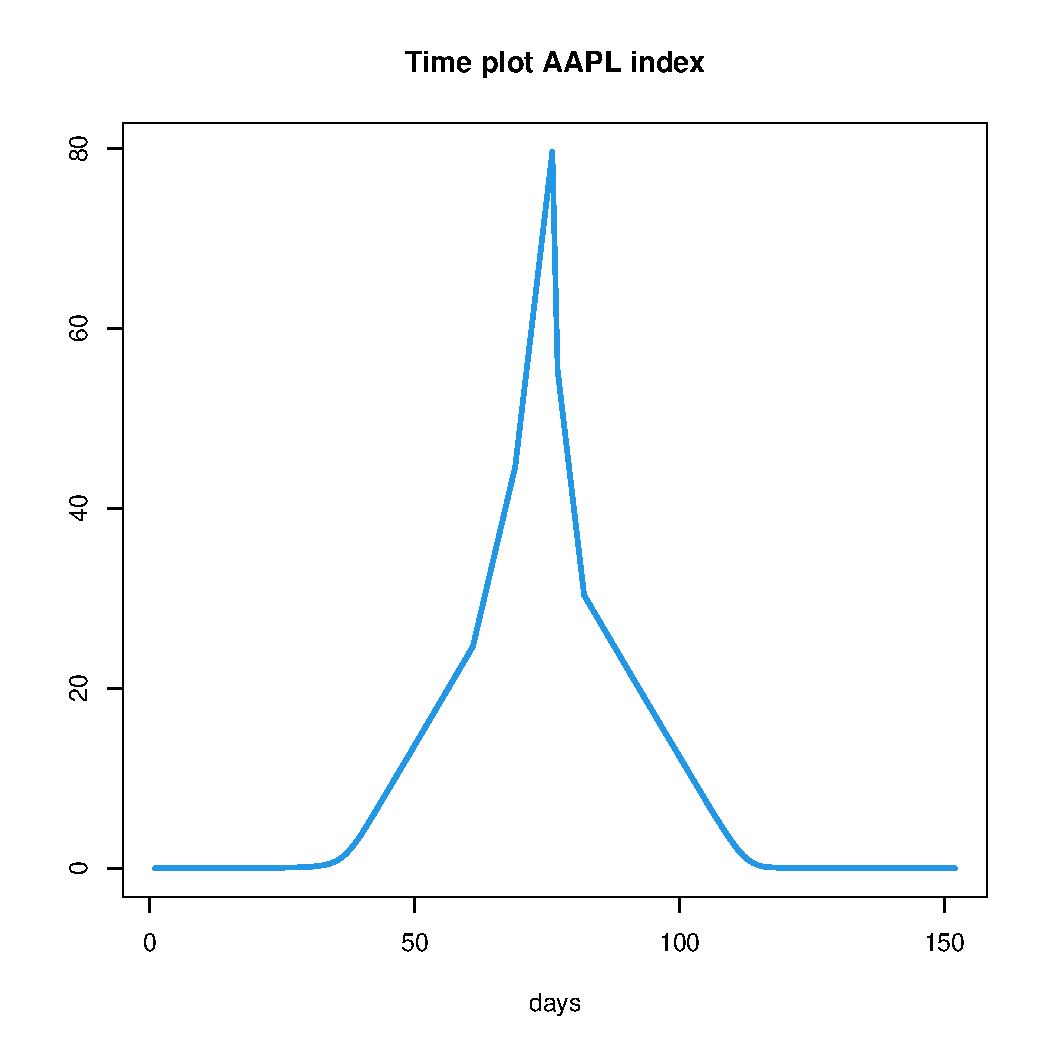
\includegraphics[width=\maxwidth]{figure/unnamed-chunk-1-1} 

\end{knitrout}

We then fit a multiple linear regression model to the data using the strike,bid and ask prices for puts and calls and estimate the parameters.The observed strike price is \$120

\begin{knitrout}
\definecolor{shadecolor}{rgb}{0.969, 0.969, 0.969}\color{fgcolor}\begin{kframe}
\begin{alltt}
\hlstd{optdata}\hlkwb{<-}\hlkwd{read.csv}\hlstd{(}\hlstr{"C:/Users/cheru/OneDrive/Documents/AAPL2.csv"}\hlstd{)}
\hlstd{pmkt}\hlkwb{<-}\hlnum{0.5}\hlopt{*}\hlstd{(optdata[,}\hlnum{5}\hlstd{]}\hlopt{+}\hlstd{optdata[,}\hlnum{6}\hlstd{])}
\hlstd{cmkt}\hlkwb{<-}\hlnum{0.5}\hlopt{*}\hlstd{(optdata[,}\hlnum{22}\hlstd{]}\hlopt{+}\hlstd{optdata[,}\hlnum{23}\hlstd{])}
\hlstd{strike}\hlkwb{<-}\hlstd{optdata[,}\hlnum{3}\hlstd{]}
\hlkwd{plot}\hlstd{(strike,cmkt,}\hlkwc{lwd}\hlstd{=}\hlnum{3}\hlstd{,}\hlkwc{col}\hlstd{=}\hlkwd{c}\hlstd{(}\hlnum{2}\hlstd{),}\hlkwc{ylab}\hlstd{=}\hlstr{"Payoff"}\hlstd{,}
     \hlkwc{main}\hlstd{=}\hlstr{"Observed European option price "}\hlstd{,} \hlkwc{xlab}\hlstd{=}\hlstr{"Strike
Price"}\hlstd{)}
\hlkwd{points}\hlstd{(strike,pmkt,}\hlkwc{cex}\hlstd{=}\hlnum{0.8}\hlstd{,}\hlkwc{col}\hlstd{=}\hlkwd{c}\hlstd{(}\hlnum{4}\hlstd{))}
\hlkwd{abline}\hlstd{(}\hlkwc{v}\hlstd{=}\hlnum{121}\hlstd{,}\hlkwc{lwd}\hlstd{=}\hlnum{2}\hlstd{,}\hlkwc{col}\hlstd{=}\hlkwd{c}\hlstd{(}\hlnum{1}\hlstd{))}
\end{alltt}
\end{kframe}
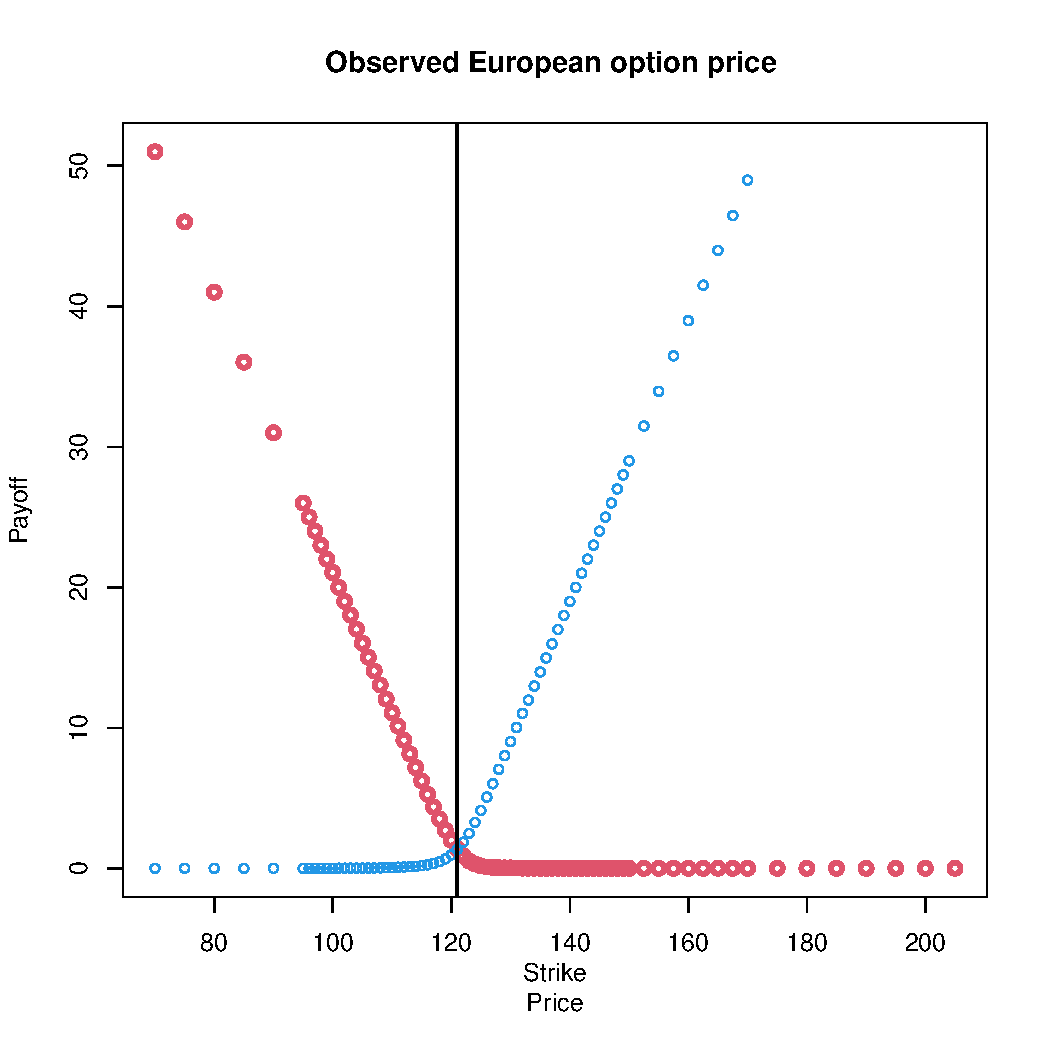
\includegraphics[width=\maxwidth]{figure/unnamed-chunk-2-1} 
\begin{kframe}\begin{alltt}
\hlstd{fit1}\hlkwb{<-}\hlkwd{lm}\hlstd{(cmkt}\hlopt{~}\hlstd{pmkt}\hlopt{+}\hlstd{strike);fit1}
\end{alltt}
\begin{verbatim}
## 
## Call:
## lm(formula = cmkt ~ pmkt + strike)
## 
## Coefficients:
## (Intercept)         pmkt       strike  
##    120.9295       0.9991      -0.9992
\end{verbatim}
\begin{alltt}
\hlkwd{summary}\hlstd{(fit1)}
\end{alltt}
\begin{verbatim}
## 
## Call:
## lm(formula = cmkt ~ pmkt + strike)
## 
## Residuals:
##       Min        1Q    Median        3Q       Max 
## -0.065045 -0.016815  0.002094  0.014834  0.035748 
## 
## Coefficients:
##               Estimate Std. Error t value Pr(>|t|)    
## (Intercept)  1.209e+02  2.380e-02    5081   <2e-16 ***
## pmkt         9.991e-01  2.921e-04    3421   <2e-16 ***
## strike      -9.992e-01  2.162e-04   -4622   <2e-16 ***
## ---
## Signif. codes:  0 '***' 0.001 '**' 0.01 '*' 0.05 '.' 0.1 ' ' 1
## 
## Residual standard error: 0.01972 on 73 degrees of freedom
## Multiple R-squared:      1,	Adjusted R-squared:      1 
## F-statistic: 1.377e+07 on 2 and 73 DF,  p-value: < 2.2e-16
\end{verbatim}
\end{kframe}
\end{knitrout}


We then checked if the the assumption of normality
over residuals is valid using the Shapiro-Wilk normality test and get the Normal QQ plot and histogram.
\begin{knitrout}
\definecolor{shadecolor}{rgb}{0.969, 0.969, 0.969}\color{fgcolor}\begin{kframe}
\begin{alltt}
\hlstd{eror}\hlkwb{<-}\hlstd{fit1}\hlopt{$}\hlstd{residuals}
\hlkwd{hist}\hlstd{(eror,}\hlkwc{probability}\hlstd{=T)}
\end{alltt}
\end{kframe}
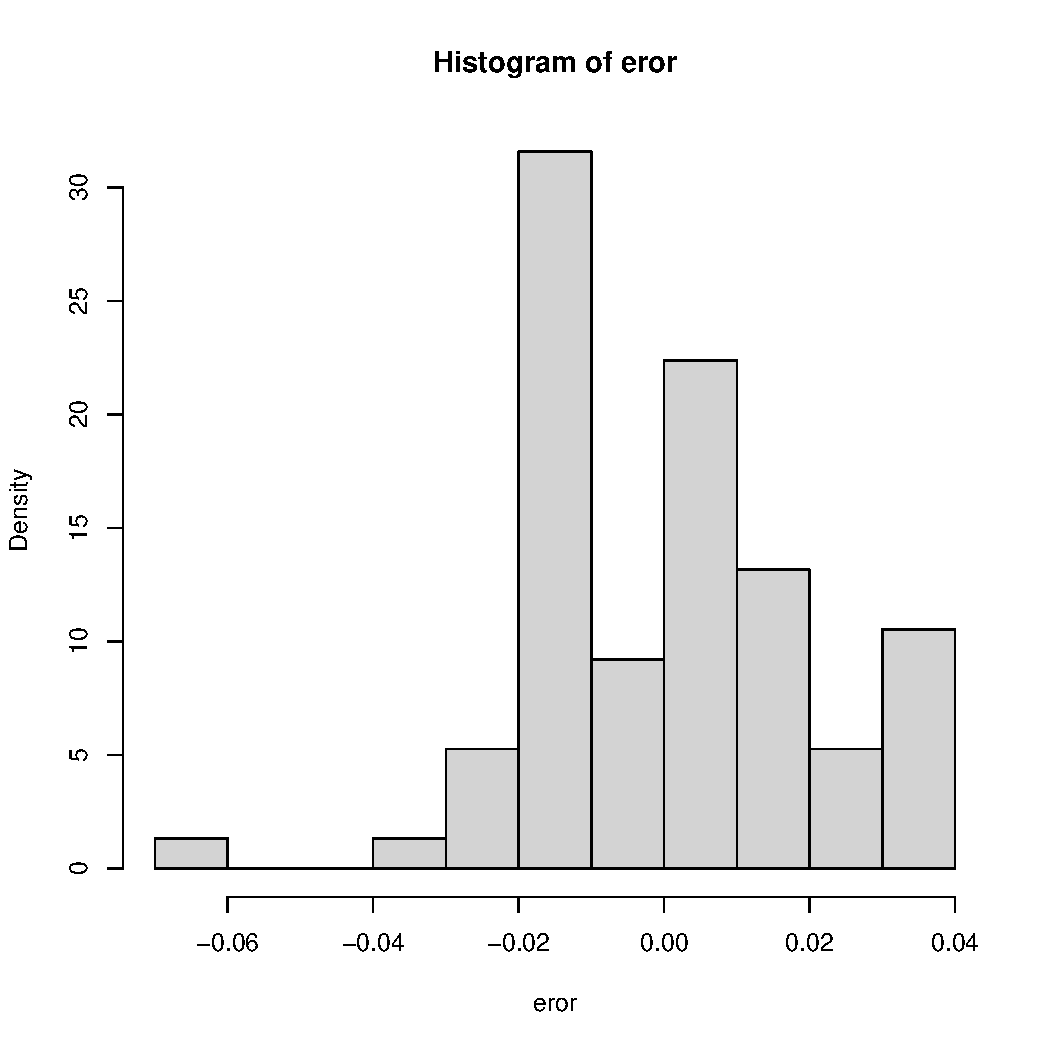
\includegraphics[width=\maxwidth]{figure/unnamed-chunk-3-1} 
\begin{kframe}\begin{alltt}
\hlkwd{shapiro.test}\hlstd{(eror)}
\end{alltt}
\begin{verbatim}
## 
## 	Shapiro-Wilk normality test
## 
## data:  eror
## W = 0.94538, p-value = 0.002593
\end{verbatim}
\begin{alltt}
\hlkwd{shapiro.test}\hlstd{(}\hlkwd{rnorm}\hlstd{(}\hlnum{1000}\hlstd{))}
\end{alltt}
\begin{verbatim}
## 
## 	Shapiro-Wilk normality test
## 
## data:  rnorm(1000)
## W = 0.99877, p-value = 0.7342
\end{verbatim}
\begin{alltt}
\hlkwd{qqnorm}\hlstd{(eror)}
\hlkwd{qqline}\hlstd{(eror)}
\end{alltt}
\end{kframe}
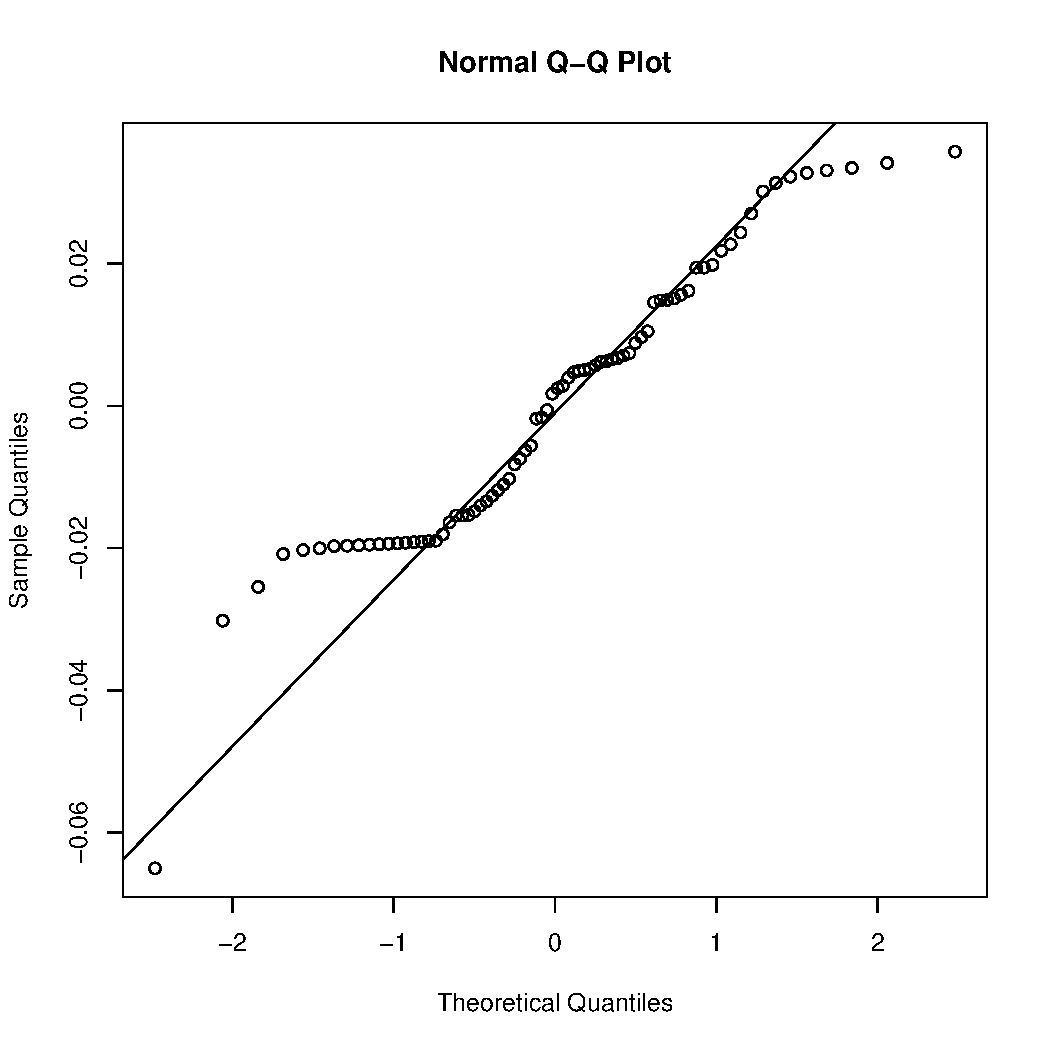
\includegraphics[width=\maxwidth]{figure/unnamed-chunk-3-2} 

\end{knitrout}

\section{Conclusion.} 
From the AAPL options chain data we have used we see proof of put-call parity after fitting a multiple linear regression model to the data.The shapiro-wilk normality test returned a p-value of 0.9839 which is greater than 0.5 thus we conclude there is indeed normality over the residuals.

\end{document}
